\chapter{Measurements and Metrological Characterization}
Several measurement campaigns were done to characterize the system.
A number of measurements were done at different solenoid tilt
angles, to estimate the effect of tilt-swing misalignment on
the peak shifts of coils. Maps with all 21 coils
were done at a number of angles, as well as repeated measurements
for accuracy estimation. A number of procedures had to be developed
in order to make the measurements repeatable.

\section{Fluxmeter Precision Estimation}
To estimate the precision and repeatability of the fluxmeter, 10
measurements were done under identical conditions. Coils D1-D5 as
well as Q44 were used since these have a large spread in total coil area.
The normalized standard deviation was then calculated for each coil.
Figure \ref{fig:coilarea} shows the standard deviation as a function
of coil area.

\begin{figure}[!h]
    \centering
    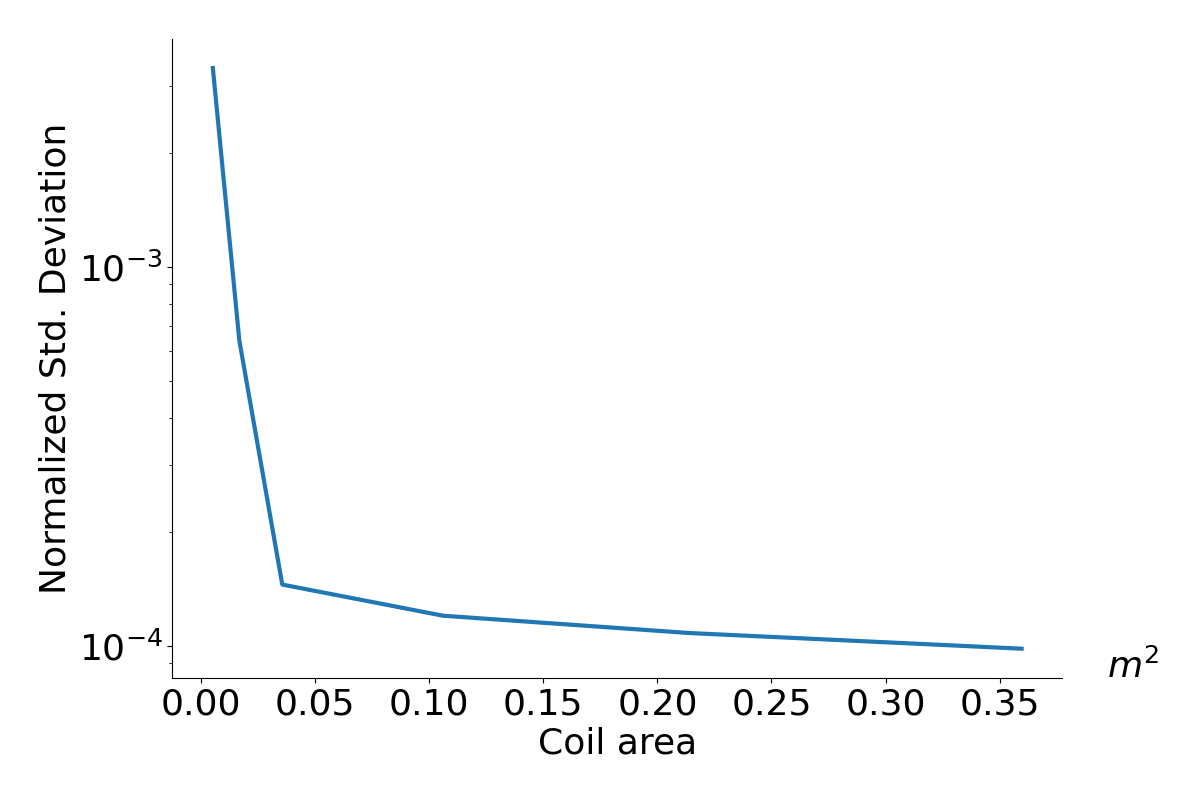
\includegraphics[width=0.8\linewidth]{figs/coilarea-error}
    \caption{Normalized measurement std. deviation as a function of
        coil area.}
    \label{fig:coilarea}
\end{figure}

As can be seen, the standard deviation of the measurements starts
increasing very fast as the coil surface area gets lower than
about $0.02$ $\text{m}^2$. A likely cause is that the signal
is starting to reach the same magnitude as the noise at this
point, which means that this is a reasonable lower bound
on the coil surface area for a magnet of this strength ($80$ mT).
For the region where the signal to noise ratio is high, the
normalized standard deviation is reliably in the low promilles.

\section{The Fluxmeter Alignment Procedure}
An alignment procedure was developed for the fluxmeter, so that
measurements could be taken in an aligned, almost ideal case
or with a desired tilt angle around the $y$ axis. This will
hereafter be referred to as the yaw angle.

First, the laser tracker is used to sample the fluxmeter positions
as it is translated through the guiding tube. These samples are then fitted to
a line in three dimensional space, as in figure \ref{fig:geomfit}.

\begin{figure}[!h]
    \centering
    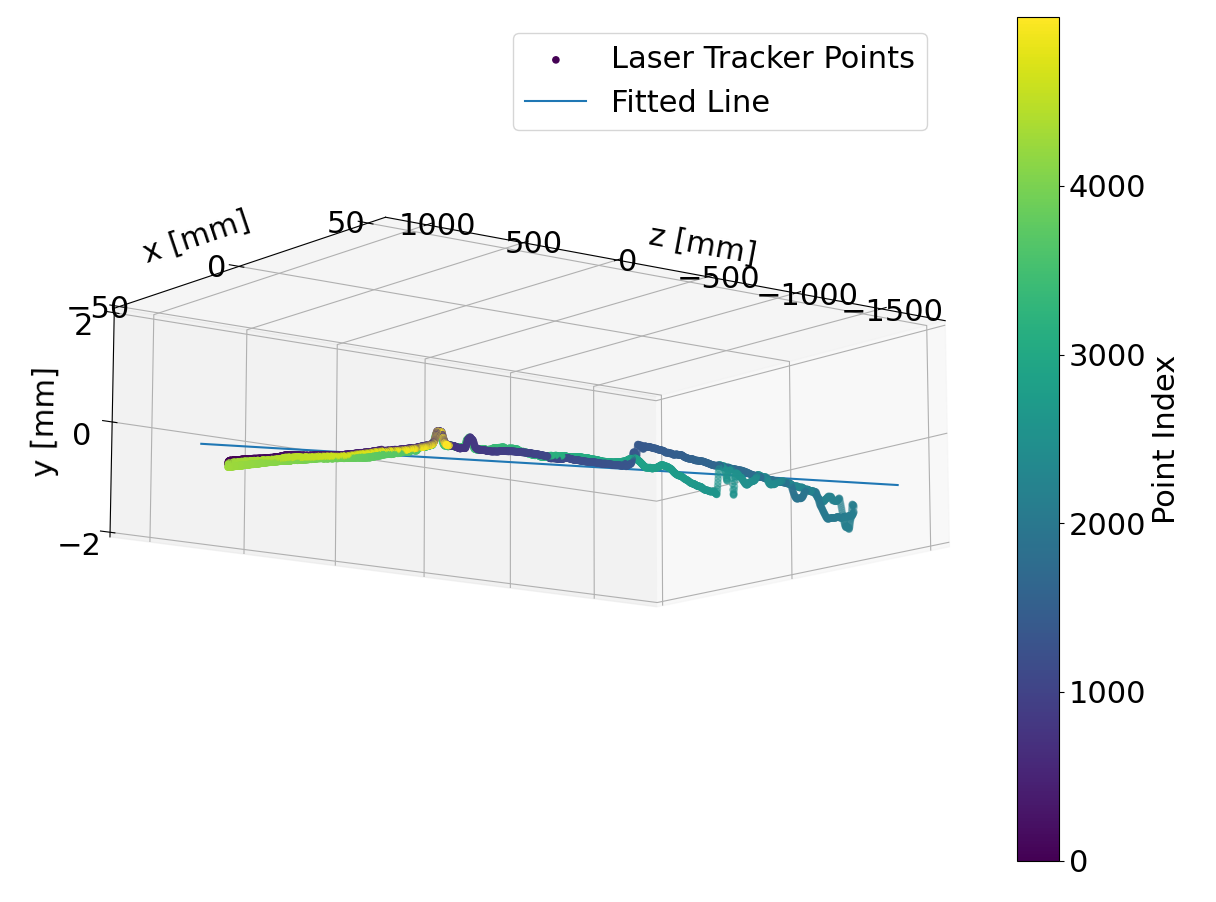
\includegraphics[width=0.8\linewidth]{figs/geomfit}
    \caption{Measured fluxmeter positions along with a line
        fit. The fluxmeter tube is tilted by $30$ mrad around the y axis.}
    \label{fig:geomfit}
\end{figure}

The intersections between the fluxmeter path line and the
planes $z = z_{Back}$, $z = z_{Front}$ are then found, where
$z_{Back}$ and $z_{Front}$ are the $z$ offsets where the tube clamps
are located. The measured intersections $\tilde{p}_1$ and $\tilde{p}_2$
are illustrated in figure \ref{fig:alignment}.

\begin{figure}[!h]
    \centering
    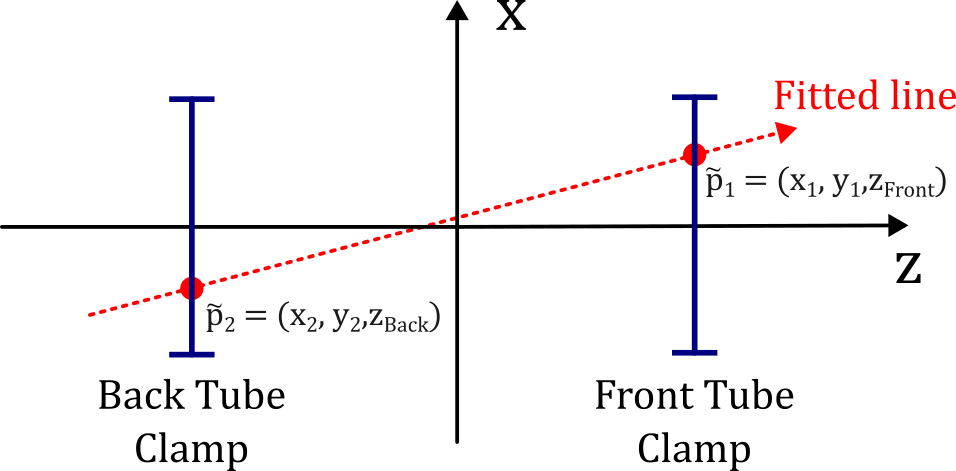
\includegraphics[width=0.8\linewidth]{figs/alignment}
    \caption{The fluxmeter path and its intersection points with
        the tube clamps.}
    \label{fig:alignment}
\end{figure}

The optimal intersect points $p_1, p_2$
are found by simple trigonometry:
\begin{align}
    p_1 = (z_{Front}\tan(\theta), 0, z_{Front}) \\
    p_2 = (-z_{Back}\tan(\theta), 0, z_{Back})
\end{align}
where $\theta$ is the desired yaw angle. Calculating the needed
adjustment is then a simple matter of comparing the measured
and optimal intersect points. The front clamp is adjusted by
$\tilde{p}_1 - p_1$ and the back clamp by $\tilde{p}_2 - p_2$.

The fluxmeter path is then measured again with the laser tracker,
and the whole procedure is iterated until the desired yaw angle
is reached, to an accuracy of
$|\tilde{p}_1 - p_1|, |\tilde{p}_2 - p_2| < 0.2$ mm.
$z_{Front} - z_{Back} = 1521$ mm, making the yaw angle error
less than $0.26$ mrad.

\section{Peak Shift Measurements}

\begin{wrapfigure}{r}{0.5\textwidth}
    \centering
    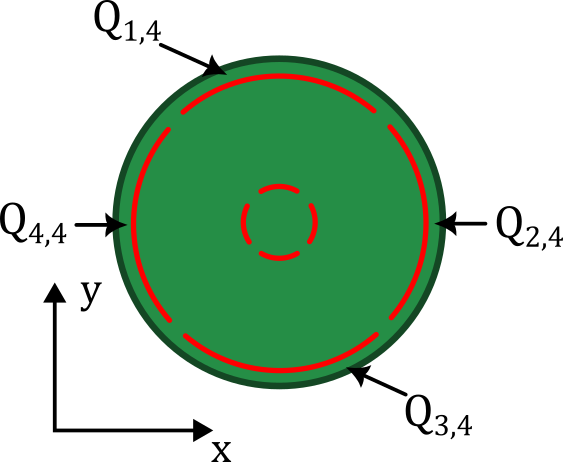
\includegraphics[width=0.8\linewidth]{figs/pcborientation}
    \caption{PCB roll orientation.}
    \label{fig:pcbalignment}
\end{wrapfigure}

As stated in section \ref{subsubsection:solenoid-harmonics},
a peak shift will occur when the solenoid is tilted relative
to the domain. To measure the effects of this, the fluxmeter
tube was yaw-tilted at seven different angles, and five
measurements were taken at each angle. The outermost
annulus segment coils $Q_{1,4}$-$Q_{4,4}$ were used for this campaign,
as well as the disc coils $D1$-$D5$. The fluxmeter was rolled
such that the Q coils were aligned with the yaw axis, as illustrated
in figure \ref{fig:pcbalignment}. With this alignment of the fluxmeter,
the expectation was that the peak shifts would be visible on the
signals $Q_{2,4}$ and $Q_{4,4}$, but not on the $D$ coils or
$Q_{1,4}$ and $Q_{3,4}$

The offsets in z at the peak field was extracted from each
measurement, the results of which can be seen in table \ref{tab:delta-peaks}
and figure \ref{fig:measured-peak-shifts}. 

\begin{table}[h!]
    \begin{center}
        \begin{tabular}{c c c c}
            Yaw Angle & $D_5$ Peak [mm] & $Q_{2,4}$-$Q_{4,4}$ $\Delta$ Peak [mm] & $Q_{1,4}$-$Q_{3,4}$ $\Delta$ Peak [mm] \\
            \hline
            0 mrad    & $0.00$          & $0.02$                                  & $-0.60$                                 \\
            10 mrad   & $-0.01$         & $0.74$                                  & $-0.44$                                 \\
            20 mrad   & $-0.01$         & $2.56$                                  & $-0.76$                                 \\
            30 mrad   & $-0.01$         & $4.29$                                  & $-0.65$                                 \\
            40 mrad   & $0.03$          & $5.95$                                  & $-0.79$                                 \\
            50 mrad   & $0.01$          & $7.30$                                  & $-0.94$                                 \\
            58 mrad   & $0.00$          & $9.41$                                  & $-0.67$                                 \\
        \end{tabular}
        \caption{Measured mean peak positions and shifts for different coils.}
        \label{tab:delta-peaks}
    \end{center}
\end{table}

\begin{figure}[!h]
    \centering
    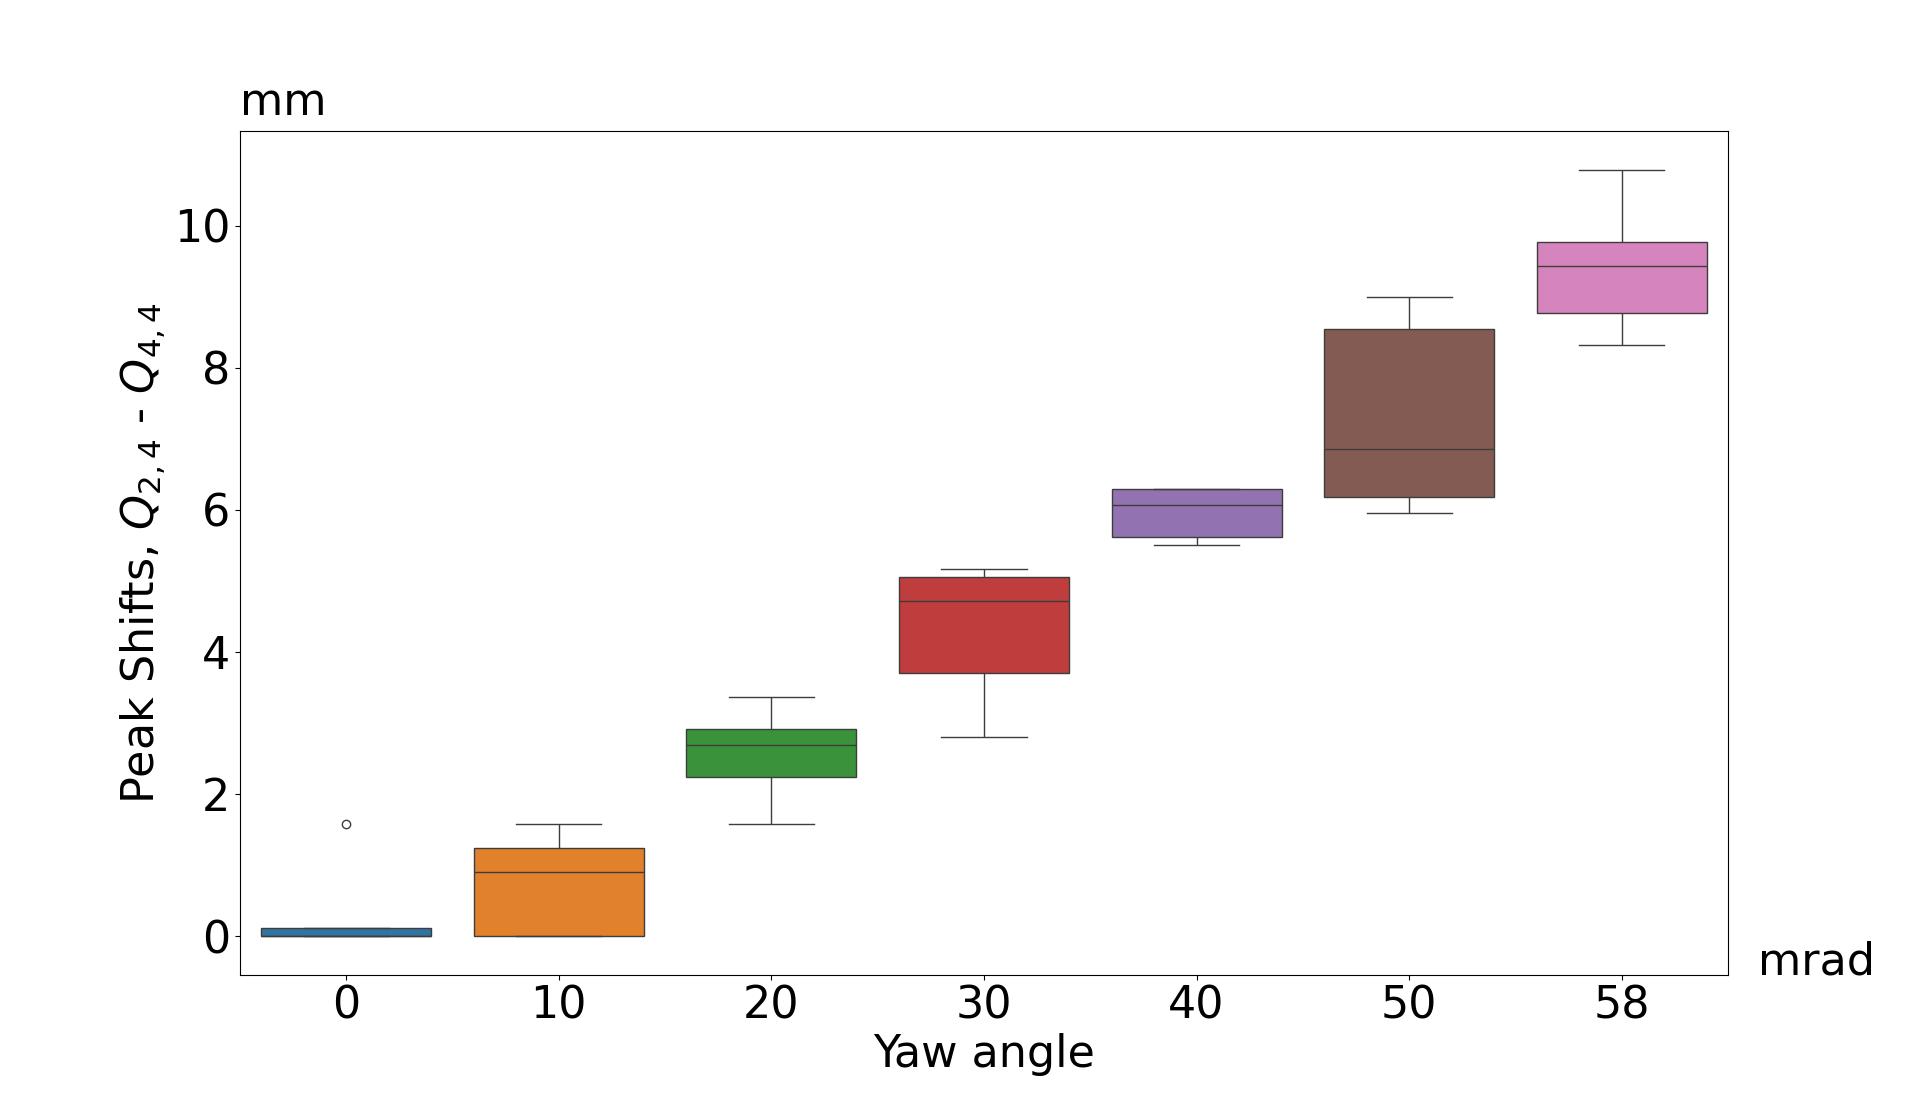
\includegraphics[width=0.9\linewidth]{figs/measured-peak-shifts}
    \caption{Peak shift between $Q_{2,4}$ and $Q_{4,4}$ as function
    of yaw angle.}
    \label{fig:measured-peak-shifts}
\end{figure}

As expected, the measured peaks only significantly shifts on the coils
that are positioned along the yaw axis. A first order linear approximation
gives a rate of $0.17$ mm peak shift per mrad. The mean of the standard
deviations of the peak shifts is $0.73$ mm. This means that the sensitivity
in the measurement of peak shifts is about $4.29$ mrad.

Next, the angle was estimated using the model presented in
section \ref{sec:project_purpose}. The peak shift $\Delta z$
and the distance $d=80$ mm was used to estimate the yaw angle,
according to equation \ref{eq:angle_estimation}.

\begin{equation}
    \theta = \arctan \left( \frac{\Delta z}{d} \right)
    \tag{\ref{eq:angle_estimation} revisited}
\end{equation}

This did unfortunately not yield very exciting results, as
can be seen in figure \ref{fig:measured_angles}. The angle
is consistently overestimated using this model. The reason 
for this was investigated in a simulation campaign, which is
presented in chapter \ref{sec:simulations}.

\begin{figure}[!h]
    \centering
    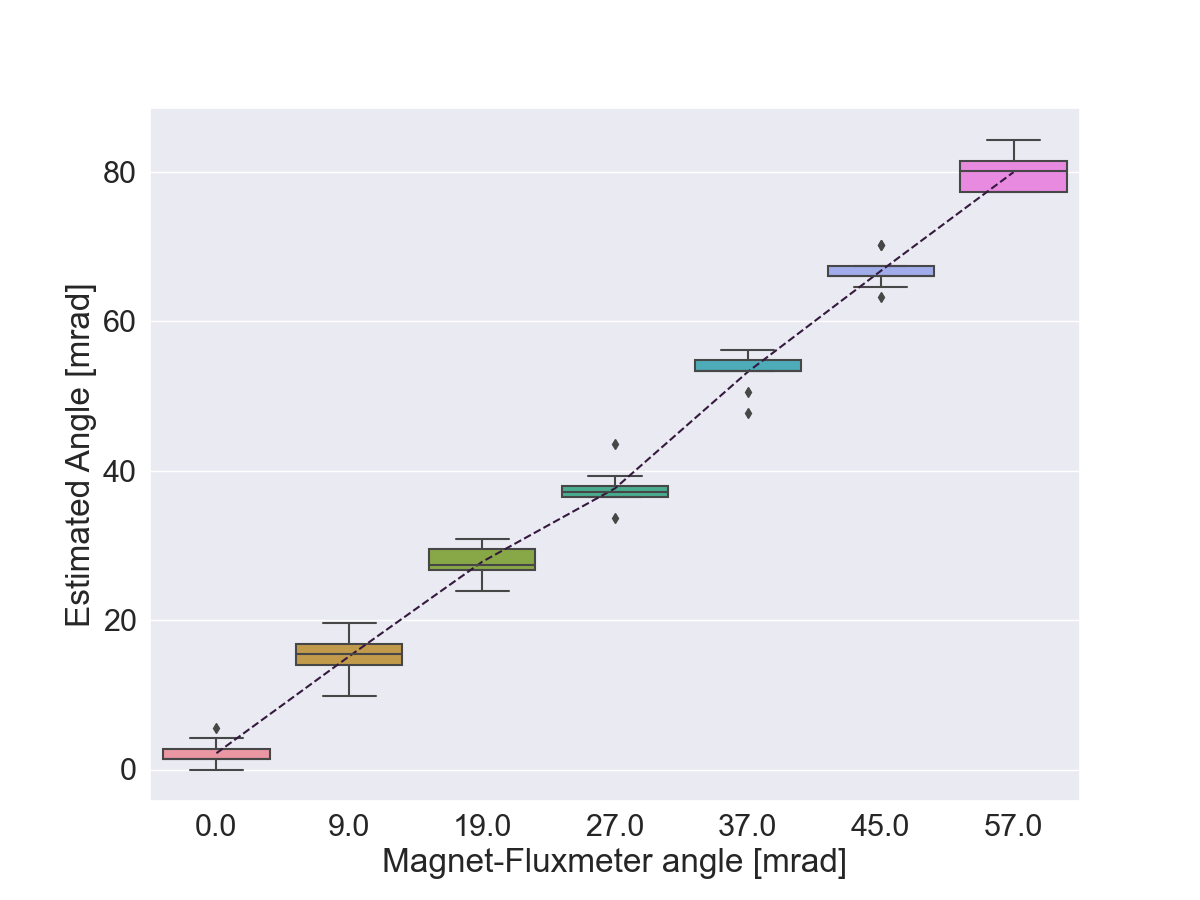
\includegraphics[width=0.9\linewidth]{figs/measured_angles}
    \caption{Estimated angles from peak shift measurements
    compared to actual angles.}
    \label{fig:measured_angles}
\end{figure}
